\chapter{Fitting Profile functions}
\label{Chap:profile}

As discussed before, to match the shapes of the peaks, you must reproduce the broadening effects of both the diffraction instrument and effects from the sample. 
What determines these broadening effects and how they are introduced into the fit will be the subject of this chapter. 

For some studies, determining the broadening characteristics is only needed as a means to obtain a good fit to the pattern, allowing determination of lattice or structural parameters, and indeed this was the original goal when Hugo Rietveld\index{Rietveld, H.} developed his eponymous analysis process. However, the parameter values that are used to model the peak profiles can provide information on the sample at the microscale, which can be very important for understanding the properties of a material that are not intrinsic to the substance but rather depend on how the substance was processed. Traditionally, microscopic techniques are well suited to provide the most detailed information on things like crystallite size and morphology, but Rietveld analysis has an advantage in that it provides measures that represent the entire sample bulk. Bulk characterization of a sample by microscopy is typically a very tedious process. The downside of sample characterization from powder diffraction is that it requires careful work to separate sample from instrumental effects.

 

\section{Peak broadening contributions convolute}

Before considering how broadening arises, it is worth mentioning that when multiple sources of broadening occur together, the each broadening contribution acts on each other in a process called convolution, which is reproduced mathematically by a convolution integral, a fairly slow computation. Use of a Fast Fourier Transform speeds this computation, because taking two functions, Fourier transforming them, multiplying the transforms together and then taking the inverse transform of the product is equivalent to performing a convolution integral, but even that is a fairly involved computation. 

 I like to think about broadening as an analogy to optical aberrations. Broadening is in effect a blurring of the peak position that comes from multiple compromises in the design of a diffraction instrument, as well as possible imperfections in the instrument, as well as defects in the sample. For those of you who, like me, must wear glasses to see well, we know that dirt on the lenses degrades our ability to see clearly. Bright sunlight, which allows the iris of our eye to become more like a pinhole camera, decreases the impact of this \textit{schmutz}. As an analogy for how broadening sources combine, consider what you see looking out a glass window. If the window glass is not uniform in thickness, then your view of the outside will be distorted where some aspects of the view will be enlarged, and others decreased in size since the window will act like a lens. If in addition, it is raining and the window is covered with rain, then the view will also be blurred, so your view of the outside will be both blurred and distorted. However, if the rain is heavy enough then the view will be so blurry that the distortions become hard to distinguish. A similar effect happens with broadening, where if we have two types of broadening that have relatively similar impact, then the two effects largely (but not exactly) add. If one broadening term is causing significant change to the signal and the other causes much less impact, then the convolution product will be only slightly changed from the more significant broadening source. 

 

\section{Sources of instrumental broadening}

So, what are the sources of instrumental broadening in powder diffraction? There are many, but let’s consider a few. First of all, how well is the wavelength determined for the probe? For conventional x-ray sources, there are usually several characteristic x-rays lines, typically labeled as Ka\textsubscript{1}, Kb, etc. These lines are fairly sharp with respect to wavelength spread, but most instruments do not isolate a single one of these lines and thus the diffraction pattern that is observed is actually a superposition from several different wavelengths. With synchrotrons and reactor-source neutrons, at least one (with synchrotrons usually a series of two or more) monochromator crystals must be used to isolate the intended radiation. A key design aspect in these instruments is how broad the wavelength range that is allowed through the monochromator, where synchrotron instruments usually transmit a very narrow portion of the radiation, with a great loss of intensity, while for reactors, the monochromator crystals are usually deformed in some fashion to transmit a much wider range of the radiation in order to retain much more of the neutron flux.

 With time-of-flight (TOF) neutrons we measure the wavelength by timing how long it takes for the neutrons to transverse the distance from the source to the detector. While a very sharp “flash” of neutrons is emitted when a pulse of protons hits a heavy metal target, these neutrons are very high energy and must be moderated by bouncing around in a material where they transfer some of their energy. Not all the neutrons will leave the moderator at the same time, and this results in a spread in the time of arrival for neutrons with the same energy. This delay effect is not symmetrical, so that TOF peaks are broadened more with neutrons arriving “late” than what would be seen if the probably for early arrival with respect to the mean time of flight were the same as late arrival. Further, since less energetic (slower) neutrons are likely to have bounced around in the moderator for longer than their higher-energy cousins, the time profile for when neutrons will arrive is narrower for higher energy (short wavelength) neutrons than for lower energy (long wavelength) neutrons; thus the resolution changes with wavelength.

 For both lab and user facilities, the spectrum of the x-rays or neutrons will never be perfectly sharp, so there is always some range in energy, which results in some broadening in diffraction peaks.

 A second contribution for aberration is the finite size of the radiation source. Remember that we need to measure the diffraction angle at infinite precision, if we want to see an infinitely sharp peak. If we do not know exactly where the photon or neutron was emitted, then we cannot know the angle of diffraction precisely. This uncertainty (equivalently, “blur”) in our peak position causes broadening. Of course, the smaller we make our source, the fewer quanta that we can measure, so the source size, like so many other aspects of instrument design, becomes a compromise between intensity and resolution. The instrument designer needs to select the intended resolution, often called the instrument response function, and then design so that each optical component in the instrument is matched to the intended resolution. If a single component degrades the resolution worse than intended, then that one factor will dominate the instrumental response. If one component alone would is set so that it would define the resolution much better than needed, it will reduce the intensity performance of the instrument with negligible gain in resolution. Thus, if we use a smaller source size, but do not improve our monochromator (or moderator) to match, we see negligible improvement in resolution but do see a significant drop in intensity. 

 The source is just one factor in the performance of an instrument. Every collimator, slit and optical component (monochromators, mirrors, etc.) will affect the overall performance of the instrument. 

 

\subsection{Low-angle peak asymmetry}

Most instrumental effects (with the exception of that from TOF moderation) creates symmetrical broadening in peaks, but there is one common effect that broadens peaks at low values of $2\theta$ and, when they can be observed, at $2\theta$ values close to 180°. In nearly all laboratory diffractometers, as well as high-resolution synchrotron instruments and CW neutron instruments, the aperture or slit that defines what radiation can be observed by the detector is elongated in this direction as well. The effect of this elongation is axial divergence. This is shown schematically in Fig.     \ref{fig:cones}
, where the x-ray or neutron beam diffracts from a small sample. Two Bragg diffraction cones are shown, one for a low angle reflection and one at significantly higher angle. Two slits are also shown schematically. The smaller one only admits the diffraction intensity at the correct $2\theta$ angle, but for the elongated slit and the lower angle reflection, the slit starts two pass intensity well below the correct $2\theta$ angle. This causes the diffraction intensity to be broadened towards lower angles, but not towards higher angles leading to asymmetry in the peak. This effect is much less severe for the higher angle Bragg cone which is why this effects lower angle peaks and falls off very quickly with angle. The same effect will occur at angles close to 180° as again the Bragg cones again have very small diameters, but the broadening is on the high-angle side. However, diffraction at such high angles is rarely possible other than with neutrons and most diffractometers already have very poor resolution at such high angles. 

\begin{figure}
    \centering
    \begin{subfigure}{0.49\textwidth}
        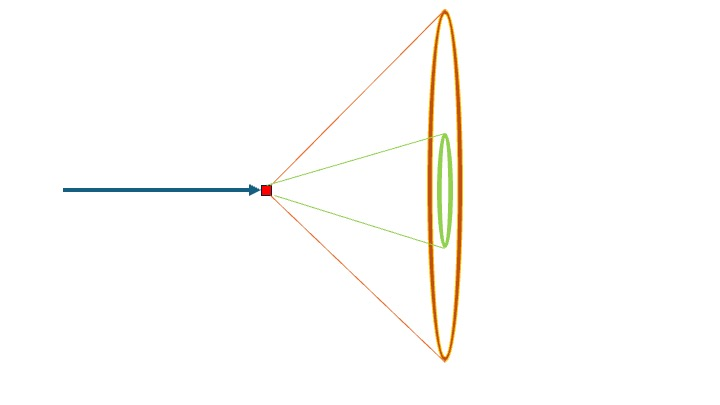
\includegraphics[width=0.9\linewidth]{figures/AxialDivergence1.jpeg}
        \caption{Side view}
    \end{subfigure}
    \begin{subfigure}{0.49\textwidth}
        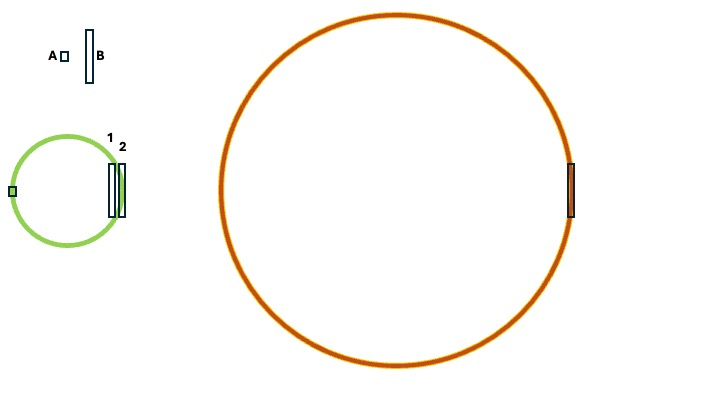
\includegraphics[width=0.9\linewidth]{figures/AxialDivergence2.jpeg}
        \caption{Viewed towards beam}
    \end{subfigure}
    
    \caption{Bragg diffraction cones for two reflections, one at low angle (green); one at higher angle (orange) viewed parallel to the diffracting beam (black arrow) and into the diffracting beam. The red square is the sample. Two slit sizes are shown. Note that the smaller slit (A) admits radiation to the detector from the low-angle cone only at the diffraction angle, but the elongated slit (B) admits radiation for the low-angle cone both at the proper angle (position 2) but also at lower angles, such as position 1. This effect is almost nonexistent for the higher angle Bragg cone.}
    \label{fig:cones}
\end{figure}

Likewise, in most instruments, the sample is also elongated in the direction of the $2\theta$ rotation circle. One can think of the effect of this as if there are a series of diffraction cones stacked along the elongation direction, as shown in Fig. \ref{fig:cones1}. This will cause the small slit to transmit radiation at angles lower than expected, thus causing approximately the same asymmetry as seen in Fig. \ref{fig:cones} with the elongated slit. Most commonly, the sample length and the slit length are matched. When both are elongated, the sample length accentuates the effect seen from the elongated slit. 

\begin{figure}
    \centering
    \begin{subfigure}{0.69\textwidth}
        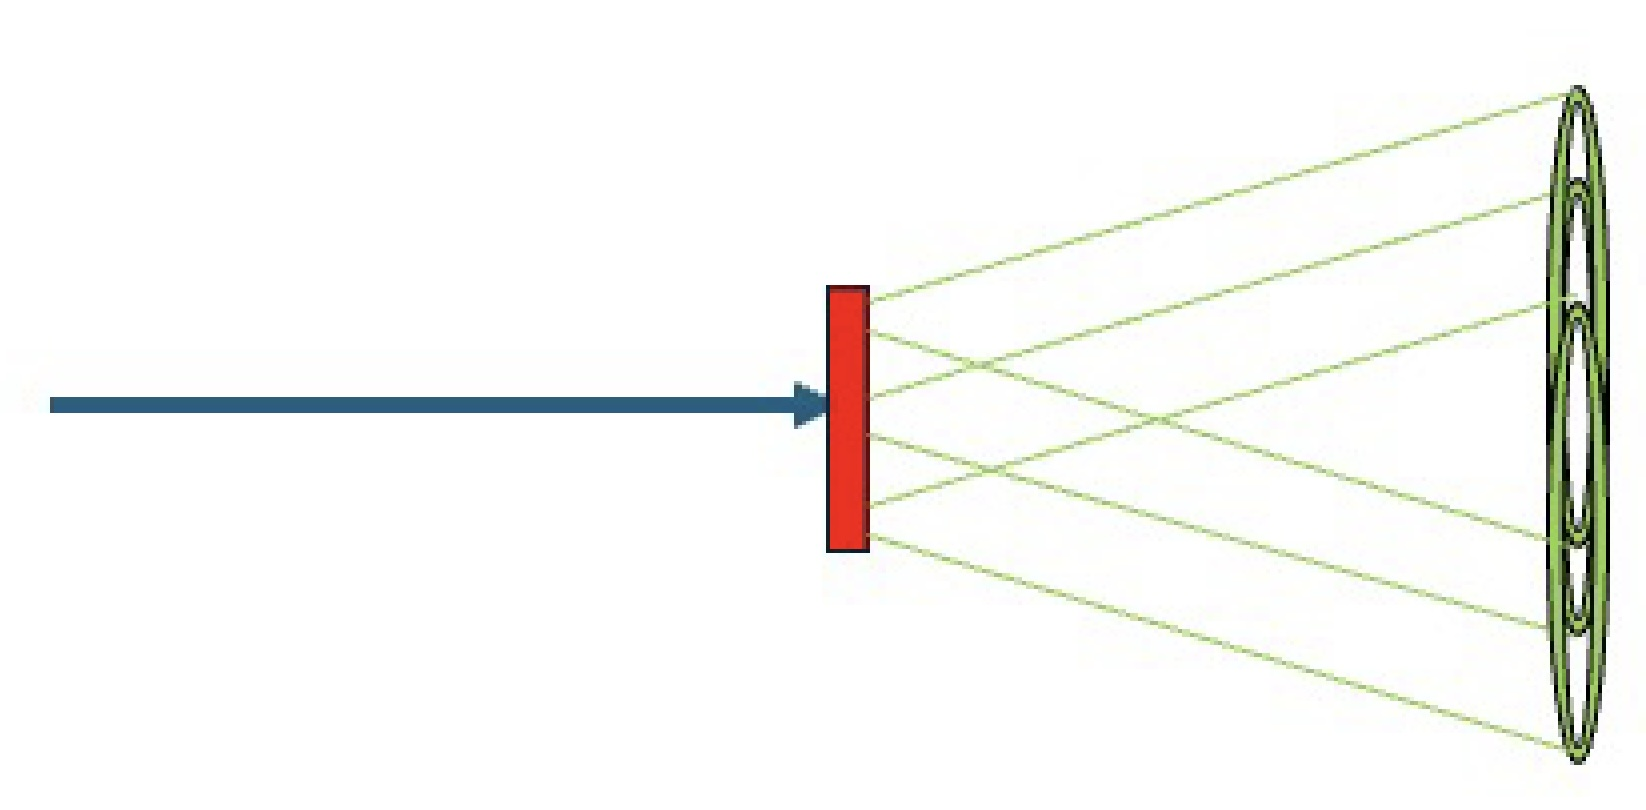
\includegraphics[width=0.9\linewidth]{figures/AxialDivergence3.jpeg}
        \caption{Side view}
    \end{subfigure}
        \begin{subfigure}{0.29\textwidth}
        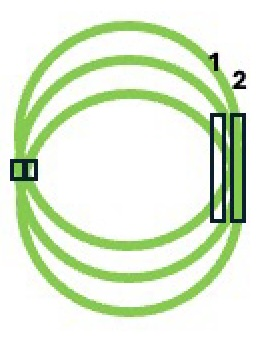
\includegraphics[width=0.9\linewidth]{figures/AxialDivergence4.jpeg}
        \caption{Viewed towards beam}
    \end{subfigure}
    \caption{Bragg diffraction cones from an elongated sample. Note that now a slit that is not elongated will see intensity at lowered $2\theta$ angles and an elongated slit sees additional intensity at low angles.}
    \label{fig:cones1}
\end{figure}

 Note that axial divergence does not occur with area detection. In such instruments the radiation source and sample sizes are minimized. The radial integration process does not cause this peak asymmetry. 

 

\section{Sample broadening}

Not only does the instrument create powder diffraction peak broadening, but all samples contribute broadening as well. While there are many types of defects in samples, such as stacking faults, screw dislocations or turbostratic disorder that can affect powder diffraction patterns, the two most significant effects are known as crystallite size broadening and microstrain broadening. Let us consider each effect. While instrumental broadening will depend only on the diffraction angle (or for TOF diffraction, both the angle and the wavelength), as we will see broadening can be different for different classes of reflections, where along some crystallographic directions, reflections will be broader than for other crystallographic directions. This is known as anisotropic peak broadening. While instrumental broadening is primarily Gaussian in nature, possibly with minor Lorentzian contributions, sample broadening is usually Lorentzian, though under unusual circumstances Gaussian contributions may be seen. 

 

\subsection{Crystallite size broadening}

As was noted in chapter \ref{Chap:diffraction}, diffraction arises from an infinite lattice of scatterers producing infinitely sharp diffraction maxima. Of course, all real crystals have finite size, so how does this affect diffraction? If we consider the diffraction from a single isolated crystal with a dimension \textit{d} (we will also consider the crystal to be spherical) then \textit{all} the diffraction maxima will be broadened in Q by a factor of 2$\pi$/\textit{d}, though the actual shape of the broadening function can be complex, particularly where \textit{d} is small, say with respect to 100*l. To relate this broadening to what is seen in measurements, we must consider that usually we measure diffraction patterns in experimental units such as an angle or for energy-dispersive measurements a unit (such as TOF) that we can relate to energy. Also, we have diffraction occurring from many crystalline domains, not one single crystalline particle, and further these domains may not be spherical. Let's consider each of these in turn.

While crystallite size causes the same broadening for all peaks \textit{measured in Q}, if we are looking at a plot of peak widths in degrees $2\theta$, we will see a change in peak widths. 
Noting that $Q = (4\pi/\lambda) \sin\theta$, the derivative dQ/d$\theta$ = ($4\pi/\lambda$) cos$\theta$. Inverting this, we see that if broadening of peaks is a constant amount $\Delta Q$, then $\Delta\theta = \Delta Q \lambda / [4\pi \cos\theta]$. Thus, crystallite size broadening, in units of $2\theta$, $\Delta 2\theta$ is proportional to $1/\cos\theta$. This broadening formulation was first developed a century ago by Paul Scherrer and is commonly written as 
$$\tau=\ {\frac{K\lambda}{\beta\cos{\theta}}}$$
where $\tau$ is the mean crystallite size in the same units as the wavelength (l); $\beta$ is the portion of full-width at half maximum of the peak that is due to crystallite broadening expressed in radians and $\theta$ is one half the $2\theta$ value for that peak. The unitless quantity K depends on the averaged morphology of the crystallites and is thus known as the shape factor. Winnie Wong-Ng in Volume H of the International Tables states that K will be in the approximate range of 0.6-2, depending on the assumption for this morphology, but is most commonly taken as 0.89. For GSAS-II we use K=1. 

\subsubsection{Anisotropic crystallite broadening}
 Note that crystallites need not have the same sizes in all directions. Anyone who has spent much time looking at powders, or for that matter minerals under a microscope knows that some materials will commonly grow with needle-like habits, where the size is much longer along one direction than in the perpendicular directions. Other materials, such as mica, may grow in a platy habit, where the length along one direction is much shorter than the perpendicular directions. With lower symmetry unit cells, many more complex unit cell anisotropic morphologies are possible. While crystallite broadening shows average properties for the entire sample that is illuminated, if the crystals have larger dimensions in some crystallographic directions than in others, we can expect to see broadening effects that differ for differing classes of reflections, since the class of the reflection (\textit{hk}0 reflections vs 00\textit{l}, for example) represent different orientations of the crystals. An easy analogy to think about the effect of orientation-dependent crystallite size on peak broadening is to imagine that the reflection “sees” the diffracting region in projection along the diffracting vector. Thus, if we consider the case where either needles or plates have their unique axis along the \textit{c} direction (this is a common case for hexagonal and tetragonal materials), we can see that the (00\textit{l}) reflections will have very different broadening from the (\textit{hk}0) reflections and the (\textit{hkl}) reflections will be intermediate between the two with the amount of broadening depending on the relative magnitudes of \textit{h}, \textit{k} and \textit{l}. In the case of needles, (00\textit{l}) reflections will be very sharp, since from that direction the crystal size is greatest. For plates, the (00\textit{l}) reflections will be very broad, since that will project as the smallest crystallite size direction. Thus, crystallite size broadening can be anisotropic when the average sizes of the crystal vary significantly by crystallographic direction. 

 Since powder diffraction is a phenomenon from a large number of crystallites and these crystallites will never all have exactly the same size, we must also consider that the distribution of crystallite sizes will convolute our size broadening. In theory it might be possible to back out the size distribution from the broadening effects and some papers have explored this, but I have not seen any convincing examples where this has been done. In powder diffraction we usually use scalar value(s) for crystallite size that represent some sort of mean value. 

 Note that I say crystallite size and not particle size here. While these terms are commonly interchanged in discussions, they mean quite different things. As an example, consider that most metal objects that we encounter are polycrystalline. (An example of an exception to that would be single-crystal titanium jet engine turbine blades.) My wedding band, for example, is a single discrete object and thus is a single particle, but it is likely composed of hundreds of thousands of crystallites. To define our terms, a crystallite is an ordered region of a material lacking long-range defects, though point defects may be present. The term grain is sometimes used for crystallite. In a somewhat circular definition, a crystallite can be considered as largest region that is seen as undisrupted ordered region by a diffraction probe, but it should be understood that different diffraction probes and even different reflections will see this differently. In contrast, a particle is a discrete object that could be a single crystal, a group of twined crystallites or even an agglomerate of randomly oriented crystallites or even could be multiphasic. Even what we call a single crystal is likely composed of multiple crystallites, since the preference for single-crystal diffraction measurements are “ideally imperfect” mosaic crystals made up of small crystalline domains that are in good, but not perfect alignment. Large non-mosaic single crystals are likely to exhibit extinction for intense reflections, which complicates structural analysis. 

 There are a number of different methods that are used for measuring particle size, which include light scattering, small angle x-ray or neutron scattering, physical separations, electrical sensing and imaging. These measure the sizes of agglomerate particles in a powder or liquid slurry. In contrast, diffraction, by x-rays, neutrons or even electrons, measures the size of the regions where atoms are scattering coherently, e.g. from a periodic lattice or even quasicrystalline domain. 

 Note that for some types of long-range faulting, some reflections may not be sensitive to the lapse in coherence caused by the fault, since in projection from a certain direction that fault might be invisible. Thus, in faulted materials some classes of reflections may be more broad than others. The faulted area might even appear to represent a longer-range structural motif in projection from certain directions and thus create new reflections that would be forbidden according to the long-range structure. This is why stacking faults can cause such complex changes in a powder diffraction pattern relative to an unfaulted material. The program DIFFaX from Treacy, Deem and Newsam, provides an excellent mechanism to model the effects of stacking faults on diffraction patterns, where a material is modeled as a set of layers where rather than having a fixed order of layering, as would be found in a fully crystalline material, probabilities are supplied for the likelihood for each type layer following the previous. GSAS-II incorporates the DIFFaX code and provides an interface for computation of faulted diffraction patterns. GSAS-II also provides visualization for the layers are joined to help prepare this relatively complex, but sometimes necessary, approach to describing a structural model. 

 When a characterization goal is to better understand the average crystallite shape or distribution of sizes, small-angle scattering is likely to be a better measurement than [wide-angle] powder diffraction. GSAS-II includes a program, Shapes, that is intended to model the mean particle size from small-angle scattering data. 

 

\subsection{Microstrain broadening}

The second type of sample broadening we will consider was historically called residual stress, but a better name for this is microstrain. To consider what this is about, let us imagine that we take a single crystal particle and put it into a C-clamp so that along one direction there is a force being applied to the crystal. For simplicity, let’s label that direction as the\textit{ c} axis. This force, which is called an external stress, will cause the \textit{c} axis to become slightly smaller since the lattice is being compressed by that force. If the same force were to be applied on the crystal uniformly, say by immersing the crystal into a container with a pressure-conducting liquid or gas and then squeezing on the container, we would then apply that force to all axes of our crystal. This would be hydrostatic stress. Thus, externally applied forces can change the lattice constants for a material. How much the lattice constants will change as a function of the force is described by a tensor populated by what are known as the elastic strain constants. The symmetry of the unit cell dictates the number of unique terms in this tensor, with 3 terms needed for a cubic system and 21 for triclinic. The name elastic stress implies that there can be a non-elastic condition. Elastic implies that if the force is released, the material will return to its original state. Indeed, if enough stress is applied, we can get outside the elastic regime. This will cause the crystal to undergo plastic deformation (think toothpaste) or catastrophic failure (cracking and breaking). 

 Now to get to back microstrain, imagine that I take a bunch of discrete unconnected crystals and put them into a container with random orientation and heat them to the point where crystals start to agglomerate, e.g. form connections to each other, but not hot enough so that the crystals start to recrystallize (where some crystals subsume others). When I remove the heat, I end up with a solid that has my crystals still randomly oriented as they started, but now the crystals are unable to move relative to each other since they are linked together. This heating process is known as sintering, but a similar process can occur when a molten material solidifies into a polycrystalline solid. Considering again our sintering material before we remove the heat, we can imagine that every crystal will have its lattice constants at equilibrium for that temperature. As the crystals start to cool, the lattice constants will get smaller, except the since there are now connections between the crystals, they are not free to shrink freely. If the contraction of the crystal lattices is at all anisotropic then some crystals will be trapped where they are unable to relax to their equilibrium lattice constants without breaking those connections. If they are unable to fully relax then they must be stretched (which we call being under strain). Since all forces must be matched, other crystals must be stress. This combination, which leads to an ensemble of crystals where there is a distribution of lattice constants, some larger than the equilibrium values and some smaller. This is the condition for residual stress. It commonly occurs in materials due to thermal and mechanical processing. 

 Microstrain broadening is really measuring the range of lattice constants in a material and there can other chemical effects that change the lattice constants for a microscopic section of a sample other than residual stress. A material may not have uniform chemical composition. The bonding of atoms close to a surface differs from that of atoms deep in the bulk (due to the truncated bonds at the surface or modified chemical environment for those atoms, should the surface be modified by oxygen or water, etc.) so the outer layers of particles may not have the same lattice constants as the bulk. 

 To consider the effect of microstrain on a powder diffraction pattern, consider the () diffraction from two crystals, one where the lattice parameter is at the equilibrium value for \textit{c}, but the other crystal has a slightly smaller lattice constant, \textit{c}-d. Recalling that $Q=2\pi d^\ast $ and for the 00\textit{l} reflections $d^\ast = l c^\ast$, we see that the reflection positions for 001, 002, 003,… reflections are, in units of Q, $2\pi c^\ast$, $2\pi c^\ast$, $2\pi c^\ast$,… If we consider the crystal that has a lattice constant of $c-\delta^\prime$, the reciprocal cell length will be $c^\ast+\delta$ and the reflection positions for those crystals will be $2\pi (c^\ast+\delta)$, $4\pi (c^\ast+\delta)$, $6\pi (c^\ast+\delta)$,… Thus, the difference in the peak positions will be $2\pi\delta$, $4\pi\delta$, $6\pi\delta$,… for Q values, $2\pi c^\ast$, $2\pi c^\ast$, $2\pi c^\ast$,… respectively. So, the spacing between the peaks from these two crystals increases as Q increases, meaning that the spacing between the peaks for each crystal is proportional to $\Delta Q/Q$. In a specimen with microstrain, we will have a distribution of lattice constants around the equilibrium value. This results in a distribution of peak positions which gives rise to peak broadening, but these peak positions also broaden proportional to $\Delta Q/Q$. 

 When looking at a diffraction pattern plotted in $2\theta$ units, we again must perform a coordinate transformation. Before we saw that $Q = (4\pi/\lambda) \sin\theta$ and $dQ = (4\pi/\lambda) \cos\theta d\theta$ so that $d\theta = (dQ/Q) (\sin\theta / \cos\theta)$ or equivalently $\Delta 2\theta$ is proportional to $\tan\theta$.

\subsubsection{Anisotropic microstrain broadening}

As noted, the range of lattice constants seen in a material can arise from multiple effects, including elastic strain. The elastic strain constants for a material can be highly anisotropic, which in other words means that a material will be much more “squishy” in some directions than others. As an example, if we consider graphite, which consists of hexagonal sheets of carbon atoms, the effect of applying pressure in the plane of the sheets would be expected to be quite different than applying pressure in the perpendicular direction to reduce the space between the sheets. Likewise, if a material has a range of compositions, the change in chemistry may well affect some lattice directions more than others. Either effect results in anisotropic microstrain broadening where some classes of reflections are affected more than others.


In conclusion, please understand that crystallite size broadening will be present in all powder diffraction samples, but it is often negligible since a diffraction instrument must have very good resolution to discern the broadening due to the size range for crystallites typically used for powder diffraction, e.g. microns; microstrain broadening will usually be present as well and it is typical for this to produce observable peak broadening. The one case where the reverse is commonly true, where crystallite size is observable and microstrain is not is in samples where very small crystallites have been created intentionally (nanoscale materials). With lower resolution instruments, it may not be possible to detect either type of broadening. Likewise, anisotropic peak broadening usually must be fairly significant to be detectable. 

The ability to differentiate crystallite size broadening from microstrain broadening depends on having discernible peaks over a sufficiently wide Q range. This is because the ability to distinguish the two sources of broadening depends on determining how that broadening changes with Q or $2\theta$. Noting that in Q, crystallite size broadens all peaks (for anisotropic broadening, in a hkl class) by the same amount, while microstrain broadening increases with Q, so that $\Delta Q/Q$ is constant. In $2\theta$ units, broadening will be proportional to $1/\cos\theta$ or $\tan\theta$, for crystallite size and microstrain, respectively. 

\section{Approaches for peak fitting functions}

Historically, there have been four different approaches used for computing powder diffraction peak profiles numerically to fit powder diffraction so that patterns may be fit. 

\begin{itemize}
\item
 One has been to use \textit{ad hoc} equations, such as the split Pearson VII function, which allows peak positions to be asymmetric because the low-Q and high-Q sides of the peak may differ in shape. 

\item
A second has been to use equations derived from physically-inspired (P-I) models. These equations are not an exact model for any instrument but are based on the underlying physics and offer adjustment factors to match performance. 

\item 
A third approach is one where a peak from the pattern is selected and then used to model the shape of all peaks in the pattern. This was developed by Christian Baerlocher\index{Baerlocher, C.} and co-workers and has been called a “learned” peak shape. It is not commonly used.

\item 
The newest method for modeling peak shapes is called the fundamental parameters approach (FPA). In this, the broadening effect from each optical component in an instrument is defined and the instrumental peak shape is determined by convoluting each of these terms, along with terms for the sample broadening. Commonly some adjustment factors are also used. 
\end{itemize}

 The \textit{ad hoc} approach for fitting is less than ideal because it can allow inclusion of effects that are not physically possible. As an example for why this is the case, the asymmetric peak broadening in low angle diffraction peaks due to axial divergence not only causes the peak to have the low-Q and high-Q sides of peaks to have different widths, but it shifts the peak positions as well. Since these shifts will not be accounted for in the \textit{ad hoc} equations, the fitting software will not compute the lattice parameters optimally. Use of learned peak shapes can handle aberrations that introduce irregular aspects to the peak shape, but it fails to handle anisotropic or Q dependent broaden effects. The greater use of machine learning techniques in recent years may mean that this approach may yet see a future renaissance. The physically-inspired approach was used in Hugo Rietveld’s initial codes and has been augmented over the decades as the basic physics description has improved. It is available in all of widely used Rietveld codes. Despite this, the FPA method has several nice features. Only a small number of codes implement FPA-generated peak shapes, but those codes are seeing wide use. If an instrument is well described, then no fitting parameters are needed to model a pattern’s peak profiles, other than for sample-related effects. The FPA method has the potential to reproduce minor deviations of the profile from the shapes produced from even the most advanced P-I functions. Creating the FPA model for a novel instrument is not a simple task, even for an FPA expert, but once done FPA fitting is unmatched for proving that an instrument is performing at the level expected for how it was designed. 

 However, my personal opinion is that the improvements in peak shape fitting from FPA for modern commercial instruments are of negligible value to improve the accuracy for the parameters derived from Rietveld analysis. For this reason, our choice in GSAS-II has been to use a physically-inspired peak shape model. It fits the profiles from laboratory instruments, as well as very specialized synchrotron and neutron instruments, well enough that the sample can be very accurately modeled and characterized; this is the goal for Rietveld analysis.

 The one valid criticism of the GSAS-II model is that fundamental parameters profile computations have the ability to describe \textit{instrumental} peak shape functions that are not well-fit by the pseudo-Voigt function that GSAS-II uses. However, modern diffraction instruments rarely have significant deviations from a pseudo-Voigt function peak shape and even where that can be noted, the contribution of the slight misfit to the model fitting results will be negligible. However, in theory with FPA one could develop sample broadening models that account for more complex treatment of sample broadening (for example, a bimodal crystallite size distribution or where defects create asymmetric broadening), but as far as I am aware no one has developed a generalized methodology for this with FPA. 

 

\section{Physically-Inspired Peak Shapes}

The forerunner to modern P-I functions was work by Caglioti\index{Caglioti, G.} et al. in 1958 (the year of my birth!) where he and co-workers characterized the instrumental resolution expected from mosaic neutron monochromators and found that broadening should be Gaussian and follow a curve where the resolution minimum is close to the monochromator takeoff angle. From this Hugo Rietveld\index{Rietveld, H.} developed a resolution curve where the Gaussian broadening function is written as $\sigma^2\ =\ U\ \tan^2{\theta}\ +V\ \tan{\theta}+W$, and this expression is now known as the Caglioti equation. In this equation, $\sigma=FWHM\ /\ \sqrt{8\ln{2}}$ ($FWHM$ is the full-width at half maximum) and $U$, $V$ and $W$ are terms determined for the instrumental configuration. This equation was not developed for x-rays, but in truth Caglioti equation is simply a polynomial and has the flexibility to fit instruments of all types. Ted Prince\index{Prince, E.} pointed out that the fitting process is much more stable if the equation is reformulated as $\sigma^2\ =\ U^\prime\ \tan^2{\left(\theta-\theta_m\right)}\ +V^\prime\ \tan{(\theta}-\theta_m)+W^\prime$, where $\theta_m $ is the monochromator “takeoff” angle. Ted was completely correct on this, but no one other than he ever implemented the modified equation in a Rietveld code. Whenever you find fitting the $U$, $V$ \& $W$ terms to be difficult, I invite you to curse the code developers (alas, I am on that list) who did not listen to Ted. 

When Rietveld analysis was initially adapted to treat x-ray data, it became clear that the pure-Gaussian peak shape initially used was inadequate for treatment of x-ray line shapes. This is because the peaks had the longer tails seen in a Lorentzian function (this is also sometimes called a Cauchy function). This is mostly because the better resolution of x-ray instruments at low angles in comparison to the neutron instruments at that time was better able to show sample broadening effects, which are largely Lorentzian. After considerable discussion in the literature, the Voigt function, which is a convolution of a Gaussian and Lorentzian function, was accepted as a good descriptor for powder diffraction peak shapes. The Voigt function is relatively slow to compute, so a substitute for this is commonly used, where a Gaussian and Lorentzian function are multiplied rather than convoluted. This produces a peak shape that is quite close to that from a similarly parameterized Voigt function. The powder diffraction community calls this product a pseudo-Voigt and it is a good approximation for the Voigt. One of my early activities in Rietveld analysis was to take a Rietveld code that used a pseudo-Voigt peak shape and add an option to instead compute a Voigt peak shape function instead. The result was a refinement that was considerably slower than the original where improvement in the fit was nearly imperceptible. My option was never used after that. 

 The commonly used form for the Lorentzian contribution to the profile is $FWHM\ =\ X\ /\ \cos{\theta}\ +Y\ \tan{\theta}$. Note that X and Y are the broadening contributions expected from crystallite size and microstrain broadening, respectively, and thus might not be the best choices for describing instrumental broadening, but these two terms together provide quite a bit of flexibility in fitting the broadening, particularly considering that Lorentzian contributions to instrumental broadening tend to be minor. As will be discussed further, below, GSAS-II introduces a third term to offer even more flexibility in the treatment of CW broadening, but it is not clear that this is ever needed. 

 One other significant improvement seen in peak shape functions was treatment for the asymmetry seen in low angle peaks due to axial divergence. The history here is that Hugo Rietveld\index{Rietveld, H.} introduced an \textit{ad hoc} correction for low angle asymmetry that did not work very well. Several other unsatisfactory treatments were tried later. The physical cause of this low angle asymmetry was well understood quite early (and is well explained in Klug \& Alexander’s 1974 book) but was first formulated in integral form in 1984 by Van Laar and Yelon, but that formalism was not conducive for peak shape computation. In 1986 Eddy\index{Eddy, M.}, Cheetham\index{Cheetham, A.} and David\index{David, W. I. F.} published a paper demonstrating that low-angle asymmetry could be fit well using the Van Laar and Yelon approach, but did not make their code available. In 1994, Finger, Cox\index{Cox, D.} and Jephcoat\index{Jephcoat, A.}, who were not then aware of the Eddy et al work, revisited the Van Laar and Yelon work, correcting some of the math. Larry Finger\index{Finger, L.}, who was a friend and prized role model to me, not only published this work, but also distributed their peak shape computation code and encouraged its employment in other software. The result is that this work is now known as the Finger-Cox-Jephcoat (FCJ) correction. While this does short-change the contribution from my very much respected friends Mike Eddy, Tony Cheetham and Bill David, I do use this naming as well; there is a moral somewhere in this about the value of putting one’s ideas into tools that others can use.

 The FCJ correction requires three parameters, the diffractometer radius (L), the length of the sample (S) and the length of the detector slit (H), where these lengths are measured along the diffractometer axis of rotation (perpendicular to the diffraction plane). The radius is used as a ratio with each of the lengths so there are really only two free parameters. These parameters in theory are known and should not need to be fit, but indeed must be adjusted when x-ray or neutron focusing is used. The two lengths have very similar effects on asymmetry and thus usually cannot be refined together. 

 These three contributions, the $U$, $V$, $W$ parameterized Gaussian function, the $X$ and $Y$ parameterized Lorentzian function, and the FCJ correction, form the backbone for P-I descriptions of peak shapes for constant-wavelength neutron and x-ray instruments in most Rietveld software, though some additional terms may be incorporated. 

 Things are quite different for TOF neutrons, which require a much more complex formulation to account for the performance of the neutron moderator, the neutron guides and path length of the instrument and the arrangement of detectors. Many different approaches have been used. The specific model used in GSAS-II was developed by my partner in GSAS-II development, Bob Von Dreele\index{Von Dreele, R. B.}, based on his unique expertise in TOF instrumentation that goes back to the initial development of the technique. Note that the parameters used to fit the instrumental broadening for a TOF instrument are determined by the facility and instrument design, which is largely fixed, though perturbations may be offered through changes in collimation options and frame selection via chopper settings. Fitting the TOF profile terms can be a tricky process, since more than one combination of values can produce comparable fits. This fitting is best done periodically by an instrument scientist, who will supply profile values along with reduced data suitable for input to a refinement. 

 

\section{GSAS-II Profile Implementation}

The creation of GSAS-II provided us with the option to rethink how profiles are handled in Rietveld. In earlier programs, such as GSAS/EXPGUI, a single set of profile terms are provided to describe both the instrumental and sample broadening effects. Even when broadening for an instrument was well-characterized, as is common for user instruments at neutron sources, the mixing of instrumental and sample contributions in the refinement stage made it difficult to discern which was which. 

 This was not a serious problem with the initial role for Rietveld fitting, where a diffraction dataset was collected (perhaps with less care than desirable for the reproducibility in the instrumental settings,) from a material that consisted primarily of a single phase and where the goal was a crystal structure determination for that primary phase. Fitting of broadening was a necessary chore, and learning the profile parameters was not typically a goal. We now use Rietveld for so many more types of measurements. When considering a more common contemporary use-case for Rietveld, we are likely to have data from a well-characterized diffractometer on a multiphase material. Rietveld is commonly employed for materials where the atomic structures are well understood, but we want to learn about materials effects, such as microstrain or phase composition or details for site substitutions or lattice constants or perhaps how the material evolves with time or the application of temperature, an external electric field, pressure, etc. From this perspective we realize that the instrumental contributions for broadening should be the same for all datasets from that instrumental configuration. Further, in the ideal case those effects will be known and will not require fitting. On the other hand, crystallite size and microstrain will not be known in advance, will be different for every phase and may change over the course of a parametric experiment. Further, more complex models for anisotropic sample broadening may be needed for some phases, but not others. From this perspective it becomes clear that one wants the ability to separate instrumental and sample broadening contributions. 

 For this reason, GSAS-II associates instrumental broadening terms with each PWDR (powder) histogram, where the initial values for the parameters are read from the instrument parameter file used when the dataset histogram is initially imported. The sample broadening terms are considered both a property of the phase (as there is no reason that two different phases would be expected to have the same crystallite sizes or microstrain) but also a property of the histogram, since the specimen used for each measurement might have differing sizes or morphologies. Thus, there are independent values for sample broadening for every histogram in every phase, so if there are $m$ histograms and $n$ phases, there will be $n \times m$ sets of sample broadening terms. Bob and I call such parameters HAP parameters (histogram-and-phase) in a name that dates back to the original GSAS program. Note that where one wishes to force sample broadening values to be the same, for example where the same specimen is used in multiple histograms, constraints can be used to group the values. These HAP parameters are placed in a location of the GSAS-II data structure associated with each phase, but there is some choice on how they appear in the GUI. This will be discussed further below.

 

\subsection{GSAS-II Instrumental Profile Treatment}

GSAS-II places the instrumental broadening terms into the “Instrument Parameters” section of each PWDR (powder) histogram. The instrumental parameters for sample broadening for CW x-ray and neutron histograms consist of U, V, and W, as described as above. For TOF neutron histograms, the peak shape is generated from convolution of double exponential and pseudo-Voigt. The exponential parameters are split between the “rise side” (shorter TOF, or equivalently high Q) and the “decay side” (longer TOF or small Q). On the low TOF side of the peak, there is one parameter a, which is multiplied by d*. One the high TOF side of the peak, there are three terms, b\textsubscript{0}, b\textsubscript{1} and b\textsubscript{q}, which are scaled by 1, d*\textsuperscript{2} and d*\textsuperscript{4}, respectively. The pseudo-Voigt is parameterized where the variance for the Gaussian contribution to the peak, $\sigma$, ($\sigma=FWHM\ /\ \sqrt{8\ln{2}}$) is determined from 
$$\sigma\ =\ \sigma_0\ +\ \frac{\sigma_1}{d^{\ast2}}\ +\ \frac{\sigma_2}{d^{\ast4}}\ +\ \frac{\sigma_q}{d^\ast}$$
and the Lorentzian contribution, g, (g = FWHM) is determined from
$$\gamma=\frac{X}{d^\ast}+\frac{Y}{d^{\ast2}}+Z$$
There are theoretical reasons for the choice of these functions, but the parameterization is largely determined from experience with a variety of TOF instruments. Most instruments do not require all these terms for a good fit, but each of these terms has been needed for a good fit for at least one instrument. 

In GSAS-II, the three terms used in the FCJ correction for low-angle peak asymmetry (S, H, \& L) are reduced to a single value (S+H)/L with S=H and this parameter is much more stable with respect to refinement.

 
\section{GSAS-II Sample Broadening Terms}
\index{HAP parameters|textbf}\label{ref:HAP}

GSAS-II offers separate terms for crystallite broadening and for microstrain and those terms can be applied isotropically or two models are provided for anisotropic broadening for each. As was noted before, there are sample broadening terms associated with each histogram for each phase, so if there are $m$ histograms and $n$ phases, there will be $m \times n$ sets of sample broadening terms. 

\subsection{GSAS-II Size Broadening Models}

For crystallite broadening, the GSAS-II offers three models, which will be discussed directly below. 

\subsubsection{Isotropic}
 The default broadening model is labeled as isotropic, which of course assumes a uniform crystallite size in all directions. This model has two refinable parameters: One is for the mean crystallite size and the second, labeled LGmix, determines if the broadening will be Lorentzian, Gaussian or a mix between the two.

 The isotropic crystallite size parameter has units of mm (10\textsuperscript{-6} m). This is determined using the Scherrer equation with a K value of unity. While K=1 does not exactly match the most common crystallite morphologies that are encountered, we consider that crystallite broadening is not a rigorously defined quantity, so while relative differences between measurements on different specimens of the same sample may be determined quite accurately, no one should ever be concerned about a discrepancy of 10\% between different quantification methods or as a difference from measurements on different materials, where the morphology may differ. Note that as the crystallite size parameter decreases, more broadening occurs, while larger values provide very minimal broadening. From a practical perspective, the instrumental resolution limits the maximum value of crystallite size broadening that can be discerned from a dataset. 
 GSAS-II does not allow the crystallite size to refine below 0.01 $\mu$m. At this value peaks are so broad as to defeat Rietveld analysis. It the size parameter also is not allowed to refine above 10 $\mu$m, which would produce imperceptible broadening with any existing powder diffractometer. In practice, with a very high resolution instrument, values above perhaps 3 $\mu$m are meaningless. More typical for most diffractometers may be 1 $\mu$m. It is the user’s responsibility to review the refined value for the size parameter and to eliminate refinement for this parameter once the value is above the discernible range for the instrument that has been used.

 The default for LGmix is 1, which means the peaks will be 100\% Lorentzian. If LGmix is 0 then the crystallite broadening would be 100\% Gaussian and values between 0 and 1 create a linear mix between the two. Physically, an LGmix value of 1 is what is expected, except from materials that have a very unusual distribution of crystallite sizes, such as a monodisperse size. While the parameter LGmix can be varied, values other than 1 seldom improves a fit. Unless a significant improvement is seen for other values, the value is best fixed at 1. Values less than 0 or greater than 1 represent peak shape functions that are highly unlikely, but I am not comfortable saying that they are always physically impossible. Seeing a value other than unity most likely indicates a problem with the background fitting, but perhaps could arise from something very unusual in crystallite size distributions. I will only change LGmix from unity if I have extreme problems in obtaining a good fit to the peak profile. 

 \subsubsection{Uniaxial}
 When there is evidence for anisotropic peak broadening and the broadening arises primarily from crystallite size, a more advanced model is that of uniaxial size broadening. This describes the average crystallite shape as a cylindrical, which in extreme cases extends to platy or needlelike morphologies. For this, one provides the crystallographic direction for the axis of the cylinder and this model provides two size parameters, axial and equatorial sizes, which again have $\mu$m units and are otherwise similar to the previous isotropic value except that the axial value is the average size value along the specified crystallographic direction and the equatorial value is the size perpendicular to that direction. There is also a single LGmix parameter to describe the Lorentzian vs. Gaussian character of the broadening, which again is rarely any value other than one. 

 Picking axes to select for broadening can be a trial-and-error process. For some Bravais lattice choices, there is only one sensible axis for broadening: For tetragonal, hexagonal or rhombohedral (hexagonal setting) the (001) axis is unique. [Note that for rhombohedral space groups in a rhombohedric setting, the (111) axis is equivalent to the hexagonal (001) axis and thus is unique.] For cubic cells, there are effectively three unique and non-perpendicular axes (001), (110) and (111). Highly anisotropic habits in cubic systems are unusual but uniaxial broadening nonetheless can be attempted to see if the fit improves. For orthorhombic, monoclinic and triclinic cells, there are no symmetry-based restrictions on preferred broadening directions, but analysis of peak widths may suggest a direction that has the broadest or narrowest widths or trial-and-error may suggest a preferred axis that improves the fit significantly. 

 \subsubsection{Ellipsoidal}
 The remaining crystallite size broadening model that GSAS-II offers is labeled ellipsoidal, as the average crystallite is assumed to have a shape described by a tensor that is analogous to the anisotropic displacement parameter (ADP) ellipsoid. The terms in the tensor are labeled by GSAS-II as S\textit{ij}. The diagonal elements (\textit{i}=\textit{j}) of the tensor specify crystallite lengths along three orthogonal axes and the off-diagonal terms (\textit{i}¹\textit{j}) orient the ellipsoid relative to the cell axes. Thus, there are six terms to refine, though one may want to start with only the diagonal terms. Note that in higher symmetry Bravais lattices, just as for ADP’s for atoms on high-symmetry sites, symmetry may require constraints, but at present GSAS-II does not force this. Thus, use of this model is not recommended for cubic, hexagonal/rhombohedral or tetragonal symmetry, unless users understand the symmetry implications on the tensor terms.

 

\subsection{GSAS-II Microstrain Broadening Models}

\subsubsection{Isotropic}
For microstrain broadening, the GSAS-II default broadening model is also labeled as isotropic, and again assumes microstrain is uniform in all directions. As is the case for isotropic crystallite size broadening, this model has two parameters: One is for the mean microstrain and the second, labeled LGmix, determines if the broadening will be Lorentzian, Gaussian or a mix between the two. 

 The microstrain parameter is the unitless quantity $\Delta Q/Q \times 10^6$. Note that this value has the opposite broadening effect from the crystallite size parameter. Smaller values produce less broadening. The default of value for microstrain is 1000, which can be considered a lower limit value for most diffractometers. (With 11-BM and other high-resolution diffractometers, one can see broadening with microstrain in the range of 300-500, perhaps). If the value decreases to a value that is insignificant, reset it and turn off the refinement of this parameter.

 The default again for LGmix is 1, which means the peaks will be 100\% Lorentzian. This parameter can be varied, but it seldom improves fits and unless a significant improvement is seen for other values, the value is best fixed at 1. I am unable to imagine what could give rise to an LGmix values less than 0 or greater than 1, but perhaps there might be physical reasons why this might be the case. Again, if I see a significant improvement in a fit when LGmix refines to a value outside the range of 0-1, I would look carefully to make sure the background fit is reasonable.

 \subsubsection{Uniaxial}
 When there is evidence for anisotropic peak microstrain broadening, the next model to try is that of uniaxial microstrain broadening, which is very much analogous to the uniaxial crystallite size broadening model. Here, this describes a system where the material is either much more stiff or much softer in one direction, particularly compared to the perpendicular directions. Again, one provides the crystallographic direction for this unique direction and again there are now two microstrain parameters, axial and equatorial, which again are $\Delta Q/Q \times 10^6$ (unitless). There is a single LGmix parameter to describe the Lorentzian vs. Gaussian character of the broadening, which again is rarely any value less than one. The same discussion for selecting a broadening axes from uniaxial crystallite size broadening applies here as well. 

 \subsubsection{Generalized}
 The third model for microstrain is labeled as “generalized” and is based on the work of Popa and Stephens to expand microstrain with symmetry-consistent Bessel function terms. The number of terms provided depends on the Laue class for the phase, but because these terms must be consistent with lattice symmetry, they usually refine with good stability. Unlike the elliptical case for crystallite size broadening, one can try fitting with the generalized microstrain model in a routine manner. 

 

\section{GUI Access to Sample Broadening Terms}

 As noted, sample broadening is treated in GSAS-II as both a property of the phase (as there is no reason that two different phases would be expected to have the same crystallite sizes or microstrain) but also a property of the histogram (since the specimen used for each measurement might have differing sizes or morphologies.) One can define constraints that force the size parameters to be the same across datasets (which might be useful where the same batch of material was used for all measurements). I have used this for impurity phases, where too few peaks to fit broadening well for all phases. By default, these “HAP” parameters are found on each Phase’s Data tab, as seen in Fig. \ref{fig:size1} where I have outlined the crystallite size values in yellow.

\begin{figure}
    \centering
    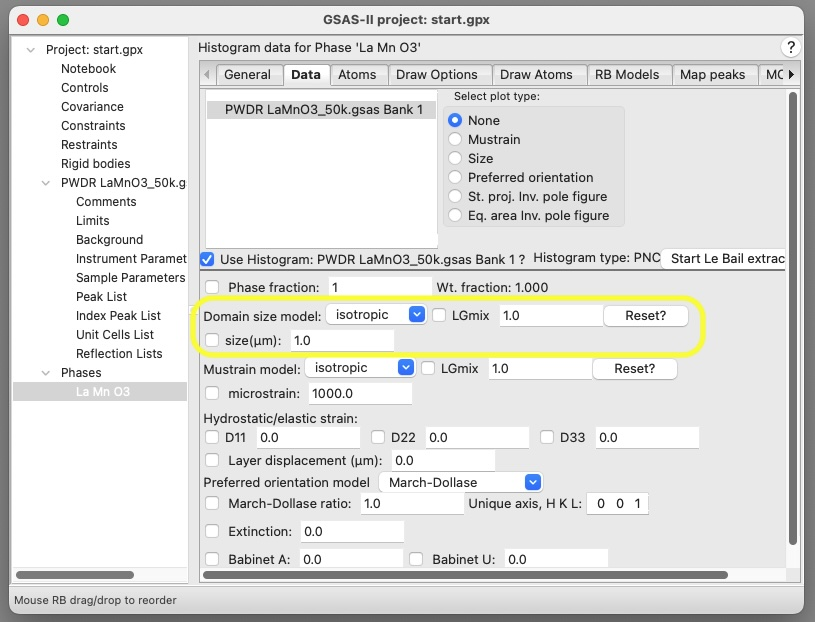
\includegraphics[width=0.75\linewidth]{figures/size1.jpg}
    \caption{Location of crystallite size parameters in the default data tab of the Phase.}
    \label{fig:size1}
\end{figure}

The phase is selected from the data tree and the histogram is selected from box to the upper left. Menu commands allow duplication of the parameter values between different histograms. Copying of values can be done where all values are copied (menu command “Copy data”) or where only selected values are copied (menu command “Copy selected data”). It is also possible to duplicate only the refinement settings (we call them refinement flags) with the “Copy flags” menu command. There is no mechanism at present for copying values between phases. 

\subsection{Placing HAP parameters directly into data tree}\label{ref:separatehistogram}

 Note that GSAS-II offers a mode where these “HAP” values are placed in their own data tree entry. (I prefer this mode.) This mode is selected using the preference variable “SeparateHistPhaseTreeItem” as shown in Fig. \ref{fig:HAPmode}. 

\begin{figure}
    \centering
    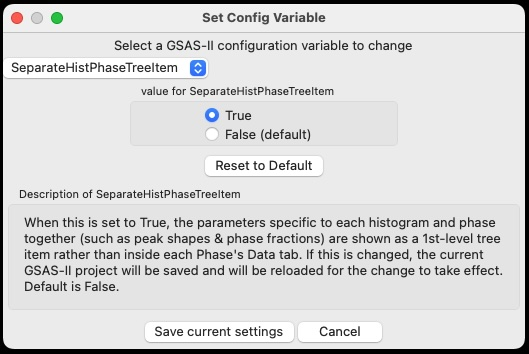
\includegraphics[width=0.5\linewidth]{figures/SeparateHAP.jpg}
    \caption{Figure 4: Setting to put the HAP entries in a separate tree entry}
    \label{fig:HAPmode}
\end{figure}

When this is done, these entries are accessed in the Hist/Phase item in the data tree and the window has a slightly different appearance (note that phases are now selected using the tabs at the top of the window), as seen in Fig. \ref{fig:size2}.

\begin{figure}
    \centering
    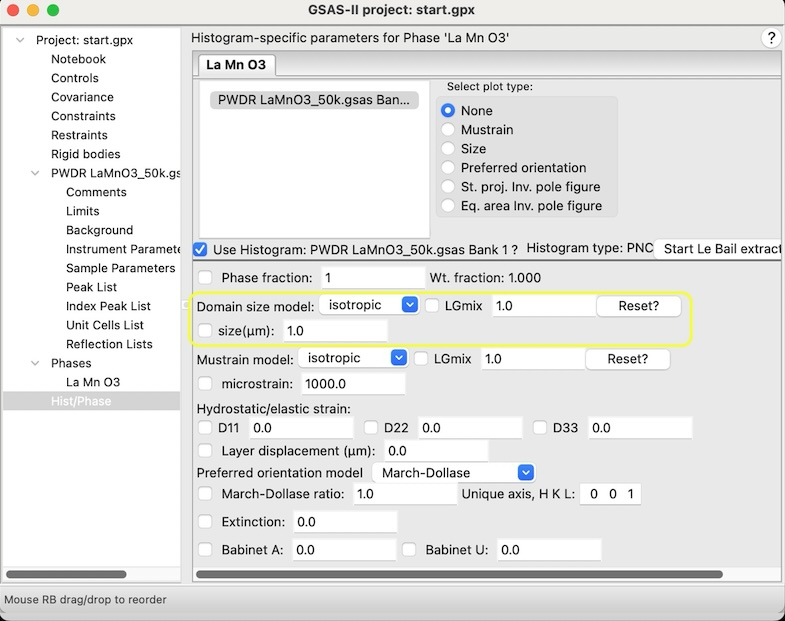
\includegraphics[width=0.75\linewidth]{figures/size2.jpg}\caption{Size parameter location with optional setting to place the HAP settings in a separate data tree entry}
    \label{fig:size2}
\end{figure}

 

\section{GSAS-II Sample Broadening Visualization}

While the isotropic crystallite size and microstrain terms have no geometric implications, interpreting the anisotropic models from the numerical values is a challenge, particularly for the third form of each set. For this reason GSAS-II allows one to visualize the model for the average for the crystallite size and microstrain values in 3-D as a function of geometry. This is done in the GUI by selecting the plot type in the upper right as “Size” for crystallite size and “Mustrain” for microstrain. For the isotropic models a sphere is plotted, but for the uniaxial case it may be of some value to visualize the relative sizes of the on-axis vs. perpendicular broadening. For the ellipsoidal case, this is more useful as it shows both the lengths and orientation of the crystallite model. The plots for microstrain fitting from the generalized Stephens/Popa model can be unusual shapes where there is considerably more microstrain in directions diagonal to crystal axes, as opposed to along the crystal axes. Since overfitting, where too many terms are introduced, is a constant concern in Rietveld analysis, it is always worthwhile to look at this plot and consider if the values make sense with what is known about the material. 

 

\section{Determining Instrumental Profile Terms}\label{ref:DeterminingInstrumental}

The preferred way that GSAS-II will be used will have these instrumental broadening terms determined for the instrumental configuration before a dataset is imported. Ideally, someone else will have carefully determined these values for you (for example at a synchrotron or neutron source, or in a well-run x-ray lab). If those values are provided to you as an .instprm file (or in the format used by the original GSAS code, where .INS, .prm and .inst are common extensions), you can read these values in with your dataset and then ignore them while you work on fitting aspect of your sample that you care about. This greatly simplifies the process of fitting diffraction data. This is especially true with TOF data where the instrumental profile terms are quite complex. 

Note that if your instrument has configuration options, such as changeable collimation (slits), a moveable detector or neutron chopper settings, these will affect the instrument resolution and the instrumental broadening terms need to match the configuration used for data collection. 

 If you do not have these instrumental broadening terms for your instrument, you are best off collecting a diffraction pattern with a standard to calibrate the instrument. You want to collect data over the same range that you will use for data collection on samples, or perhaps a wider range. The standard should have sharp peaks over a wide angular range and ideally should have known crystallite sizes and microstrain. The NIST Standard Reference Material 660 (LaB\textsubscript{6}) is an excellent choice for this, particularly the 660c version, which is made with \textsuperscript{11}B, so that it can be used for neutrons as well as x-rays, but is expensive -- if it can even be located for purchase. Some samples of Na\textsubscript{2}Al\textsubscript{2}Ca\textsubscript{3}F\textsubscript{14} (commonly called NAC) have been produced that have even sharper peaks than NIST LaB\textsubscript{6}. Silver behenate [CH\textsubscript{3}(CH\textsubscript{2})\textsubscript{20}COOAg] is commonly used for sharp lines at low diffraction angles. Many inexpensive materials can be obtained that produce sharp diffraction peaks with minimal microstrain and crystallite broadening, but often these materials have small unit cells and do not diffract at low angles. However, scans of multiple materials to provide diffraction peaks at low as well as high angles or even a mixture could provide an inexpensive secondary standard for diffraction line profiles. Work on this would be very useful to the community. Measurement and fitting of data on standard(s) for an uncharacterized instrument has the additional advantage that it demonstrates that the instrument is performing well. If a standard cannot be well-fit, then it is quite unlikely that more complex studies can be completed with better results, as there is an instrument alignment or problematic performance issue (such as x-ray tube contamination). 

 After collecting data on a standard, one should read the data into GSAS-II. The GUI will then ask you to provide an instrument parameter file, but if you do not have one with reasonable parameters, you can press “Cancel” on that dialog and a second window will offer choices with default options. 

 Fitting profile terms to data for a standard can be a surprisingly difficult task when starting from values well away from an optimal set. GSAS-II provides two tutorials\footnote{GSAS-II tutorials can be viewed using the Help/Tutorials menu command or at web page \url{https://advancedphotonsource.github.io/GSAS-II-tutorials/tutorials.html}}  
 ``Create Instrument Parameter File: Determine Starting Profile from a Standard”
 for a laboratory instrument and 
 ``Calibration of a Neutron TOF diffractometer” that run through the process of this fitting. Note that optimal profile term fitting requires that the background, lattice constants and peak intensities all be well fit, in addition to the peak profiles. If, for example, the background is too low in the region of some peaks, then profile fitting will tend to widen peaks and artificially increase the Lorentzian contribution to the peak(s) so that the peak tails contribute to what should be modeled as background scattering. 

 Note that instrumental broadening is typically Gaussian and sample broadening Lorentzian, so when fitting the instrumental terms, the X \& Y terms should initially be set to zero and only U, V \& W be refined for CW instruments. Non-zero values for X \& Y are rare and if refined, this should be where the crystallite size and microstrain values are set to known values. One should never refine X \& Y and either the crystallite size or microstrain together. 

 

\section{FPA Generation of Instrumental Terms}

If the diffraction instrument’s optical properties are well characterized, then it is possible to construct a description of the expected peak profiles using the fundamental parameters approach (FPA). While FPA models have been developed for synchrotron and neutron diffractometers, this is primarily the domain of laboratory x-ray diffractometers. GSAS-II provides a module where FPA terms may be input and an automatic process then 

generates peak profiles as a function of $2\theta$ and fits them with the GSAS-II profile coefficients. These profile terms are then used to generate an instrument parameter file. The FPA profiles are generated with the NIST ``Fundamental Parameters Python Code'' from Marcus H. Mendenhall et al. that is included in GSAS-II. To access this capability, use the “Fit instr. profile from fundamental parms” command in the Powder Diffraction submenu in the Imports menu; also see the ``Determining Profile Parameters with Fundamental Parameters'' tutorial. 


\section{How to Refine Peak Profiles for a Sample}

There are three usual cases for how peak profiles might be fit with GSAS-II: 

\begin{enumerate}
\item The preferred case, where the instrument is well characterized and only sample terms need to be refined. 

\item Where one must work with a dataset without known instrumental broadening terms. 

\item Where an instrument is being characterized to determine the instrumental broadening terms. 
\end{enumerate}

The third case has been discussed previously in the “Determining Instrumental Profile Terms” section, \S\ref{ref:DeterminingInstrumental}. The second case is to be avoided wherever possible, but will be discussed further, below. So, I will first consider the process for fitting the sample broadening terms when the instrumental terms have already been determined for the instrument configuration used for data collection, which is what I would prefer to see people do. Good fits for peak profiles are only possible when the peak locations (from lattice parameters and sample displacement parameters), background and reflection intensities are all well fit. Thus, there are four interlocking aspects of Rietveld fitting. Please be sure to read the chapters on peak position (Chapter \ref{Chap:peakpositions}), background (Chapter \ref{Chap:background}), and peak intensity fitting (Chapter \ref{Chap:intensities}) before attempting to fit sample broadening.

\subsection{Refinement of sample terms only}

The optimal way that GSAS-II profiles will be fit will be to use previously determined profile terms that accurately describe the instrumental contribution to peak profiles. When this is the case then a good fit for the observed peak profiles should be obtained with refinement of the sample terms and the instrumental broadening terms do not need to be fit for samples. This greatly simplifies the Rietveld fitting process. In very simple cases, it will be possible to refine the histogram scale factor, background, lattice parameters and sample broadening all at the same time, but when any of those parameters start fairly far from their optimum values, the refinement may move to unreasonable values for some parameters and once that happens further optimization may not be possible. For this reason, I recommend a more systematic approach where parameters are added to the model in a more deliberate sequence. 

 Note that for complex crystallographic studies, where the starting model will not fit the diffraction intensities well (since improving an inaccurate model is the point of the study), it will not be possible to fit peak profiles well with the starting model; but it may also be impossible to fit the crystallographic structure with a poorly-fit peak shape. One approach to this is to cycle between fitting the background, then the peak shape, then the structure, (while also optimizing the unit cell parameters) and keep returning to each of these and possibly adding new parameters, such as sample displacement and preferred orientation, in turn until an optimum fit has been obtained. To remove intensity fitting from the combined tasks for fitting all aspects of the data, some researchers perform an initial profile fitting using a Le Bail\index{Le Bail fitting} or Pawley\index{Pawley fitting} fit (see \S\ref{ref:LeBail}), where peak intensities are optimized directly, rather than have them determined from atom positions, preferred orientation etc. I recommend this approach. The steps used for this can vary, but here is a good recipe to follow: 

\begin{enumerate}

 \item \textbf{Refine the scale factor} alone, or optionally with the background terms before starting the Le Bail/Pawley fit. The reason for this is that later in the refinement, when you turn off the Le Bail/Pawley fit, if the scale factor is very far from correct, other parameters (particularly peak shape and lattice) may refine to quite incorrect values prior to the scale factor converging. These parameters should return to their optimal values in subsequent refinement cycles, but this does not always happen.

 \item \textbf{Fit the background}. How this is best done depends on the complexity of the background. It may be sufficient to refine a few Chebyshev terms, or one may need to define fixed background points and fit background peaks to them. This will depend on the sample. See the Background Fitting chapter (Chapter \ref{Chap:background}) for more details on different approaches to fitting background. 

 \item Once the background is well fit, \textbf{fit the lattice parameters}. Before doing this, confirm that the structural parameters place computed peaks in positions that overlap with the observed. If they don’t the likelihood is that the refinement will not progress. If using Pawley fitting, refine only the intensities of the peaks for a few cycles before refining lattice parameters. With Le Bail, this should be done for you when you perform your first refinement after setting turning the Le Bail setting on. (One can also fit the Le Bail intensities alone by running a refinement after setting the number of least-squares cycles to zero.) Don’t forget to include the refinement of the appropriate sample displacement parameter(s) for the type of instrument and sample you are using. See the Lattice Parameter Fitting chapter (Chapter \ref{Chap:peakpositions}) for more details

 \item \textbf{Confirm} that the \textbf{background and lattice} are well fit: At this point the difference curve should be relatively flat and close to zero, except in the regions where peaks are found. [Using the “w” option to view (obs-calc)/sigma can help considerably in seeing this is true.] Likewise, the computed peaks should be well-centered with the observed peaks. Look for the “derivative shape” in the difference pattern when observed and computed peaks are not aligned. 

 \item Try refining the \textbf{isotropic broadening }parameter. Should that be the isotropic microstrain or crystallite parameter? My GSAS-II coauthor Bob’s comments on this are valuable: “…ask yourself about how the sample was made. If hand-ground, the size will not usually be small enough to cause broadening, but there will be lots of microstrain that could be complex. If the sample is a precipitate or has been annealed, then the size \& microstrain may be both “ideal” \& cause little broadening at all. Nanomaterials (by definition) will have size broadening but unknown (\& probably difficult [impossible] to determine) microstrain because of the broad peaks. Always apply the ‘Occam’s Razor’ principle \& look for the simplest model that fits the data.”

 For this reason, I suggest starting with the isotropic microstrain parameter except for nanomaterials, where the crystallite size makes more sense. The microstrain value starts with a default of 1000 and should not be refined if it drops below a value that is insignificant for the instrument that has been used. Should this happen, reset it and turn off the refinement of this parameter.

\item While it is fairly rare to have data over a wide enough Q range to \textbf{refine both crystallite size and microstrain together}, I will often try this to see if it is possible. Usually, I save the refinement under a new name prior to doing this, so that it is easy to discard the fit with both parameters refined together after it goes awry. Note that while small values of microstrain produce insignificant broadening, large values for the size parameter are insignificant. The default value for the size parameter, 1 micron, is insignificant for most diffractometers so a value any larger is an indication of a problem, but 11-BM can show broadening of a few microns. Again, reset and turn off the fit for a parameter that refines out of a reasonable range, but unless you have prior information that a very small-grain sample is in use, or note that a fit with size alone gives a significantly better fit than microstrain alone, microstrain broadening is more plausible than crystallite size alone and as such is a more reasonable model. 

 \item \textbf{Try uniaxial anisotropic broadening} for whichever parameter is providing the greatest broadening contribution if refinement of broadening is significantly improving the fit. While one might expect it to be fairly clear from the difference plot that some peaks are wider than others, in practice I often discover anisotropic broadening is present only because the fit improves significantly only when I try this option. The uniaxial model, which changes the number of terms from one to two is sufficient for testing for this improvement, and the default broadening axis of 001 is the best choice for most high-symmetry systems (111 for rhombohedric cells), but for orthorhombic, monoclinic or triclinic systems it may well make sense to also try other axes. If the ratio of the fit metric (R\textsubscript{wp} or GOF) before-and-after the addition of the extra parameter only changes by a few percent or less then the two broadening values are likely quite close and anisotropic broadening is not improving the model – return to an isotropic model. 

 \item If uniaxial microstrain broadening improves the fit significantly, try refining with the \textbf{generalized microstrain model}, particularly for higher symmetry systems. I have seen good fits with monoclinic cells, but I would not attempt this with a triclinic structure with less than superb data with plenty of widely separated peaks. If this does not produce a significant improvement in the fit (the ratio of the fit metric before-and-after the addition of the extra parameters changes by less than a few percent), return to the uniaxial model. Also, before deciding to use this model, particularly if the fit improvement is small considering the number of parameters that are added, look at the plot for the microstrain surface and see if the directions where there are the greatest and least deviations in the lattice parameters and see that it makes chemical sense from the structure. If the broadening is predominantly from crystallite size, I do not suggest use of the generalized crystallite broadening mode, unless you are sufficiently knowledgeable to know which terms are consistent with the symmetry of your lattice. 

 \item Once the profile terms, background and lattice parameters are determined well from a Pawley or Le Bail fit, if one is faced with a complex crystallographic analysis, where the process will be more complex than just turning on the refinement flags for a few atoms, for example where interstitial or charge-balancing atoms may need to be located, it can be helpful to stop these terms while exploring structural options. When turning off the Le Bail/Pawley fit, make sure to turn on the refinement of the histogram scale factor. If the scale factor is far from correct (this can be checked by running a zero-cycle fit), it is best to refine for a cycle this before varying any other parameters. Once the crystallographic parameters have been well-fit, for a final refinement run, do return the profile terms, background and lattice parameters back into the fit. 

 \item For some datasets it is not possible to refine the peak shape, ADP’s ($\rm U_{iso}$ values) and background together. This is discussed in detail in \S\ref{ref:negativeUiso}. This happens where the data has so many peaks at high Q that there are no areas far enough from reflections so that there is Bragg intensity in every data point over a wide region. When this is the case it may be possible that there is no unique minimum for the optimum $\rm U_{iso}$ values along with the background location. As will be discussed further, if the high-Q background is placed too low, then more intensity is needed in high Q reflections, which causes $\rm U_{iso}$ to be set to values lower than the real value. My solution for this is to fix all the U\textsubscript{iso} values to a value somewhat larger than I would expect, based on my experience for the material type and data collection temperature, and then fit the background and sample broadening but not $\rm U_{iso}$ parameters. I then stop fitting the background, but do fit the U\textsubscript{iso} values again. At this point the U\textsubscript{iso} values will typically refine to larger values than what I had before. When you publish the work, do note that this was done and why. 

\end{enumerate}

Note that while usually I recommend fitting sample broadening only after fitting the lattice and background, when the peaks in the data are much more broad than the instrumental resolution, it can be difficult to fit the lattice and background well when the peak shapes are very poorly fit. (The reverse should never occur where the computed peaks are more broad than the observed pattern!). Looking at the “Rietveld plot” which shows the observed and computed patterns and their differences, particularly for peaks where intensities are well fit will demonstrate how well the peak widths in the fit match the data. In this case, it may be useful to refine either a single size or microstrain value (which one it is not overly important) so that the peak shape is close to correct before working out the details on how to model the background. Once the background is well-fit the process above can then be followed. 

 When it is not clear to me which model I want to use, I will frequently set up two refinements, for example, one with a microstrain term, and one with a crystallite size term, or an isotropic model compared to the uniaxial model, to see which gives a larger drop in the GOF, reduced c\textsuperscript{2} or R\textsubscript{wp} values. I will then compare the two fits and continue with the refinement that provides the largest improvement and discard the other. If no significant drop is seen in either refinement in comparison to the default value, then sample broadening is not significant. It may show more improvement if attempted later in the final stages of the refinement when all other parameters are fit, but if then the fit does not improve, do not include sample broadening in the final fit and note when publishing that negligible sample broadening was observed. If both terms provide fairly large, but similar fit improvements then it is possible that both types of sample broadening are present, but unless the data presents discernable peaks over a wide range of Q, it is quite possible that the two terms have more-or-less equivalent effect on the fit. 

 As noted, it is possible to make a trial refinement where both isotropic crystallite size broadening and microstrain broadening are refined together. If this is done, it should be confirmed that two things occur before continuing refinement with both terms: (A) the fit should be significantly better with both terms than with either alone and (B) the values should make sense, in that a very small microstrain value or a very large crystallite size value means that the term is not changing the peak widths and can be removed. Continue to monitor the values as even though the refinement starts with reasonable values, as while the initial fits to these parameters may have reasonable values, but this may not persist as the refinement progresses. 

 

\subsection{Refinement of instrumental profile terms}

GSAS-II can still be used with the “old fashioned” approach for fitting profile parameters in a CW fit, where U, V, W, X and/or Y are refined, but my recommendation would be to refine U, V \& W for the histogram and microstrain (or rarely crystallite size) for each sample. If your high-school best friend offers you powder diffraction data from her newly discovered room-temperature superconductor and asks you to confirm the structure using Rietveld, you will want to use that data, no matter that you do not have profile calibration data or an instrument parameter file for her diffractometer. On the other hand, one hopes that every TOF pattern will have calibration information, as TOF data is pretty much impossible to fit without instrument parameters or data on a standard that allows their derivation. 

 While under usual circumstances it is not possible to refine the sample broadening at the same time as the diffractometer X and Y terms, there are occasions where this can be done. In a multi-phase fit one might refine X \& Y for the histogram and then refine microstrain (or size, probably not both) for all but one phase. Note that if this is done, the refined microstrain/size values should be interpreted as being on an arbitrary scale, but it is possible to compare values obtained for the different phases. Since the refined sample parameters cannot make peaks sharper than the values dictated by X \& Y, in a multiphase sample, the phase with the sharpest peaks is the one that should have the sample terms fixed. Alternately, set the sample broadening terms to have non-negligible crystallite or microstrain broadening for the phase where these terms will not be fit, so that the other phases can have sample broadening terms that can be smaller than those of the fixed phase. It is also possible to refine uniaxial microstrain or generalized microstrain, even though X \& Y are being refined. Having said this, if you are in the compromised situation where data must be fit without the ability to calibrate the instrumental broadening, I think it is much simpler to leave X \& Y as zero and refine only the sample broadening terms. 

 

\section{Constraints on broadening terms}

There may be occasions where profile parameters will be refined but should have the same values for several histograms. A good example of this might be where multiple samples are used for characterization of the instrumental broadening, for example to extend the Q range of the fitting. While each histogram has a separate set of instrumental parameters, constraints can be created to force the parameters to have the same values. 

Likewise, if the same specimen is used with multiple diffraction measurements, it can be reasonable to constrain a phase’s sample broadening term(s) to be the same for all the histograms. Note that some thought should be made first to know that the measurements really do probe the exact same material. For example, a multigram neutron specimen and microgram synchrotron specimen might come from different synthesis batches and might have different crystallite sizes or microstrain values. Even when taken from the same bottle, the sampling may not be homogeneous. Use constraints with care and it is a very good idea to try a refinement where the constraint is removed. Without the constraint, parameters may refine to inappropriate values, but if the constraint is valid the fit without the constraint will not be significantly better than the constrained fit. 

 

\section{The Warren-Averbach Method}

 Back in the days when a slide-rule constituted state-of-the-art computation, the Warren-Averbach method was developed to differentiate crystallite size and microstrain broadening contributions to powder diffraction profiles. The gist of this method was that one could measure the half-width of peaks directly from the powder diffraction pattern. (Back then, most were recorded by a chart recorder directly onto rolls of graph paper, so this would be a manual task.) The values were then plotted in such a way that the slope of the width function provides a microstrain estimate and the intercept provides an estimate of the crystallite size. Note that these values still needed to be adjusted to account for instrumental contributions. I have seen discussions where the Warren-Averbach is elevated as the classical and fundamental sample broadening characterization methods that all others should be validated against. I do not agree. Its real value was that the simplicity of the computations was such that it could be done in the days prior to the availability of a pocket calculator. 

 I feel that the Warren-Averbach approach has long been superseded by profile fitting. The sample characterization mechanism provided in GSAS-II, where peak widths are generated from sample broadening terms, as well as previously-characterized instrumental contributions, is far more accurate, in that instrumental contributions are directly accounted for and offers more advanced models, in that anisotropic sample broadening can be considered. 

 

\section{Parting words on Profile Fitting}

 Powder diffraction crystallography pioneer Peter Stephens once joked that a Rietveld refinement is never perfected, but merely is abandon. This is because once one has found a good fit, there are a seemingly infinite number of things that can be attempted to make the fit better. Most will not. Nonetheless, it is worthwhile checking the sample profile models to see if a better fit can be obtained by adding a small number of parameters. One can test if LGmix refinement improves the fit. Revert to the previous model if not. Likewise, I have sometimes been fooled by good fits where I thought I was done, but I was surprised to see them improve further when I included anisotropic microstrain (irony here:) using Peter Stephen’s microstrain model. Again, check to confirm that microstrain and crystallite size broadening can or cannot be refined together. Sometimes this will not be stable in the early stages of the fit, but will work well once the structural and background parameters have reached good minima, sometimes things seem to start well, but end up with values that don’t make sense. 
